\section{Fourier methods}
\thispagestyle{plain}

Derivatives in normal space turn into multiplications in Fourier space - we can converted
a PDE into an algebraic equation by Fourier transform. Other applications of Fourier
methods are

\begin{enumerate}
    \item calculate correlation functions
    \item projection of vector operators
    \item diagonalize circulant matrices
    \item image smoothing
\end{enumerate}

\subsection{Convolution problems | solving Poisson's equation using Fourier methods}
We want to solve Poisson's equation
\begin{equation}
    \text{gravitational } \vec{\nabla}^2 \phi = 4\pi G\rho, \quad \text{electrostatics } \vec{\nabla}^2 \phi = - 4 \pi \rho
\end{equation}
for a given density distribution $\rho$ (charge density in electrostatics) (here in CGS units).

\idea{The solution to the Poisson equation is generally a convolution\footnote{A convolution of a Greens function and the density.},
which by the convolution theorem becomes a multiplication in Fourier space - a very fast operation $\mathcal{O}(N)$. So the main cost
is the Fourier transform, which can be done in $\mathcal{O}(N \log N)$.}

\subsubsubsection{The solution to the Poisson equation is a convolution}
For a point source $q$ at the origin, the density distribution is $\rho(\vec{x}) = q \delta(\vec{x})$ and we know the
potential to be $\phi = \frac{q}{|\vec{x}|}$, so in the Poisson equation $\vec{\nabla}^2 \frac{1}{|\vec{x}|} = -4\pi \delta (\vec{x})$.

As of the linearity of Poisson's equation, the solution to a more complex charge distribution is
\begin{equation}
    \phi(\vec{x})=\sum_{i=1}^N \frac{q}{\left|\vec{x}-\vec{x}_i\right|} \quad \underbrace{\rightarrow}_{\text{continuous limit}} \quad \phi(\vec{x}) = \phi(\vec{x})=\int \frac{\rho\left(\vec{x}^{\prime}\right)}{\left|\vec{x}-\vec{x}^{\prime}\right|} d \vec{x}^{\prime}
\end{equation}
or in the gravitational case
\begin{equation}
    \begin{gathered}
        \phi(\vec{x})=-G \int \frac{\rho\left(\vec{x}^{\prime}\right)}{\left|\vec{x}-\vec{x}^{\prime}\right|} d \vec{x}^{\prime}=\int g\left(\vec{x}-\vec{x}^{\prime}\right) \rho\left(\vec{x}^{\prime}\right) d \vec{x}^{\prime}=g \star \rho \\
        \text{Greens function of gravity } g(\vec{x}) = -\frac{G}{|\vec{x}|}
    \end{gathered}
\end{equation}
- \textbf{the solution for the potential is the convolution of the density and the Greens function $g$.}

\subsubsubsection{A convolution in real space turns into a multiplication in Fourier space}
The Fourier transform of the convolution of two function is equal to the product
of the individual Fourier transforms of those functions (\textbf{convolution theorem}).

\begin{equation}
    \mathcal{F}(f \star g)=\mathcal{F}(f) \cdot \mathcal{F}(g), \quad \text { functions } f, g, \quad \text { Fourier transform } \mathcal{F}
\end{equation}

We can turn a convolution in real space into a simple point-by-point multiplication in Fourier space. Applied
to the Poisson problem, we get

\begin{equation}
    \phi=\mathcal{F}^{-1}[\mathcal{F}(g) \cdot \mathcal{F}(\rho)], \quad \text { in Fourier space } \mathcal{F}(\phi)=: \hat{\phi}(\vec{k})=\hat{g}(\vec{k}) \cdot \hat{\rho}(\vec{k})
\end{equation}

\subsubsubsection{For periodic boundaries, the Fourier transform turns from an integral to a sum}

Assume our space to be a box of size $L$ in all dimensions and the boundary conditions to be periodic.

As of the periodic boundary conditions, the set of possible $k$-vectors is discrete, as illustrated in figure \ref{fig:periodic_poundaries}.

\begin{figure}[ht]
    \centering
    \includesvg[width=0.9\textwidth]{figures/periodic_boundaries.svg}
    \caption{The set of possible $k$-vectors is discrete for periodic boundary conditions.}
    \label{fig:periodic_poundaries}
\end{figure}

\begin{equation}
    \begin{gathered}
        \rho(\vec{x})=\sum_{\vec{k}} \rho_{\vec{k}} \exp (i \vec{k} \cdot \vec{x}) \\
        \text{periodic boundary conditions } \rightarrow \vec{k} \in \frac{2 \pi}{L}\left(\begin{array}{l}n_1 \\ n_2 \\ n_3\end{array}\right), \quad n_1, n_2, n_3 \in \mathbb{Z} \\
        \text{as of } \rho \in \mathbb{R} \, (\rho^* = \rho) \rightarrow \hat{\rho}_{\vec{k}}=\hat{\rho}_{-\vec{k}}^{*}
    \end{gathered}
\end{equation}

We have an infinite but discrete grid in reciprocal space.

The Fourier transform over the periodic density in real space is

\begin{equation}
    \label{eq:fourier_rho}
    \hat{\rho}_{\vec{k}}=\frac{1}{L^3} \int_V \rho(\vec{x}) \exp (-i \vec{k} \cdot \vec{x}) \, d \vec{x}, \quad \text { normalization } \frac{1}{L^3}
\end{equation}

\textcolor{blue1}{\textbf{General properties of the periodic Fourier series:}}

\begin{equation}
    \begin{gathered}
    \text { orthogonality } \frac{1}{L^3} \int_V \exp \left(-i\left(\vec{k}-\vec{k}^{\prime}\right) \cdot \vec{x}\right) d \vec{x}=\delta_{\vec{k}, \vec{k}^{\prime}}, \\
    \text { closure } \frac{1}{L^3} \sum_{\vec{k}} \exp (i \vec{k} \cdot \vec{x})=\delta(\vec{x})
    \end{gathered}
\end{equation}

\subsubsubsection{Solution to the Poisson equation in Fourier space}
Replacing the density and potential by their corresponding Fourier series in
the Poisson equation - assuming periodic boundaries - yields
\begin{equation}
    \begin{gathered}
    \vec{\nabla}^2 \sum_{\vec{k}} \phi_{\vec{k}} \exp (i \vec{k} \cdot \vec{x})=4 \pi G \sum_{\vec{k}} \hat{\rho}_{\vec{k}} \exp (i \vec{k} \cdot \vec{x}) \\
    \rightarrow \phi_{\vec{k}}=\mathcolor{green1}{-\frac{4 \pi G}{\vec{k}^2}} \hat{\rho}_{\vec{k}}=\mathcolor{green1}{g_\vec{k}} \cdot \hat{\rho}_{\vec{k}}
    \end{gathered}
\end{equation}
where $\mathcolor{green1}{g_\vec{k}}$ is the Greens function of the Poisson equation
in periodic fourier space.

\subsection{Discrete Fourier Transform (DFT)}
\greenbox{Periodicity in space led to discrete wave vectors $\vec{k}$, discretization in space will limit the different $\vec{k}$ necessary to fully represent a density distribution,
leading to a discrete Fourier and inverse Fourier transform by summation.}

On a computer, the density and potential in normal space are also
discretized to the following positions

\begin{equation}
    \begin{gathered}
    \vec{x}_{\vec{p}}=\frac{L}{N}\left(\begin{array}{l}
    p_1 \\
    p_2 \\
    p_3
    \end{array}\right)=\frac{L}{N} \vec{p}, \quad \text { box length } L, \quad \text { points per dimension } N, \\
    p_1, p_2, p_3 \in\{0,1, \ldots, N-1\}, \quad \rho_{\vec{p}}=\rho\left(\vec{x}_{\vec{p}}\right)
    \end{gathered}
\end{equation}

Using $d\vec{x} \rightarrow \left( \frac{L}{N} \right)^3$ the integral for 
calculating the Fourier transform of the density (eq. \ref{eq:fourier_rho}) turns into the sum

\begin{equation}
    \hat{\rho}_{\vec{k}}=\frac{1}{N^3} \sum_{\vec{p}} \rho_{\vec{p}} \exp \left(-i \vec{k} \cdot \vec{x}_{\vec{p}}\right)
\end{equation}

\subsubsubsection{The spatial discretization (and periodicity) limits the number of $\vec{k}$ vectors that lead to possibly different $\hat{\rho}_\vec{k}$}

\begin{equation}
    \vec{k} \in \frac{2 \pi}{L}\left(\begin{array}{l}
    n_1 \\
    n_2 \\
    n_3
    \end{array}\right) \xrightarrow[\text { discretization of space }]{} \vec{k}=\frac{2 \pi}{L}\left(\begin{array}{l}
    l_1 \\
    l_2 \\
    l_3
    \end{array}\right)=\frac{2 \pi}{L} \vec{l}, \quad l_1, l_2, l_3 \in\{0,1, \ldots, N-1\}
    \end{equation}

\bluebox{\textbf{Why does a longer range of $l_1, l_2, l_3$ not introduce additional modes?}:
Consider the inverse Fourier transform
\begin{equation}
    \label{eq:ifmodes}
    \rho(\vec{x}) = \sum_\vec{l} \hat{\rho}_\vec{k} \exp{(i\vec{k}_\vec{l}\cdot x_\vec{p})}
\end{equation}
with $\vec{x}_\vec{p} = \frac{L}{N} \vec{p}$. Consider now we would introduce a
further $\vec{k}$ to the sum with e.g.
\begin{equation}
    \vec{k}=\frac{2 \pi}{L}\left(\begin{array}{l}
        l_1 + N \\
        l_2 \\
        l_3
    \end{array}\right)
\end{equation}
then it will indeed not add a \textbf{new} mode to the sum \ref{eq:ifmodes}, as
\begin{equation}
    \exp{\left(i\left(\frac{2\pi}{L}l_1 + \frac{2\pi N}{L} \right) \frac{L}{N} p_1 \right)} = \exp{\left(i \frac{2\pi}{L}l_1 \frac{L}{N} p_1 \right)} \underbrace{\exp{\left(i \frac{2\pi N}{L} \frac{L}{N} p_1 \right)}}_{ = \, 1}
\end{equation}
\textbf{A finite number of wave vectors is sufficient to discribe a density distribution on a discretized grid - higher \textit{frequencies} are aliased to lower ones.}
}

\subsubsubsection{Resulting discrete Fourier transform}
\begin{equation}
    \boxed{
    \begin{gathered}
    \text { Fourier space } \hat{\rho}_{\vec{l}}=\frac{1}{N^3} \sum_{\vec{p}} \rho_{\vec{p}} \exp \left(-i \frac{2 \pi}{N} \vec{l} \cdot \vec{p}\right) \\
    \text { Real space } \rho_{\vec{p}}=\sum_{\vec{l}} \hat{\rho}_{\vec{l}} \exp \left(i \frac{2 \pi}{N} \vec{l} \cdot \vec{p}\right) \\
    \vec{l}, \vec{p} \in\left(\begin{array}{l}
    \{0,1, \ldots, N-1\} \\
    \{0,1, \ldots, N-1\} \\
    \{0,1, \ldots, N-1\}
    \end{array}\right)
    \end{gathered}
    }
\end{equation}
where (in 3D) we invertibly and linearly map $N^3$ values $\rho_\vec{p}$ to $N^3$ values
$\hat{\rho}_{\vec{l}}$.

\subsubsubsection{Different conventions for the wave vector $\vec{k}$ and Nyquist frequency}
The wave vectors $\vec{k}$ (in the general context of DFT also called \textit{frequencies}) are conventionally
defined as

\begin{equation}
    \vec{k}=\frac{2 \pi}{L}\left(\begin{array}{l}
    l_1 \\
    l_2 \\
    l_3
    \end{array}\right)=\frac{2 \pi}{L} \vec{l}, \quad \mathcolor{green1}{l_1, l_2, l_3 \in\left\{-\frac{N}{2}, \ldots,-1,0,1, \ldots, \frac{N}{2}-1\right\}}
\end{equation}

\note{This does not make a difference compared to $l_1, l_2, l_3 \in {0,1,\dots,N-1}$ as shifts by $\frac{2\pi N}{L}$ in an entry of $\vec{k}$ do not lead to new unique modes.}

This shift makes the occurence of positive and negative wave vectors explicit
and the $\vec{k}$-vectors are now arranged quasi-symmetrically around 
$\vec{k} = (0,0,0)^T$, as illustrated in figure \ref{fig:wave_vectors}.

\begin{figure}[ht]
    \centering
    \includesvg[width=0.9\textwidth]{figures/wave_vectors.svg}
    \caption{The wave vectors $\vec{k}$ are conventionally defined as
    $\vec{k}=\frac{2 \pi}{L}\left(\begin{array}{l}
    l_1 \\
    l_2 \\
    l_3
    \end{array}\right)=\frac{2 \pi}{L} \vec{l}$ with $l_1, l_2, l_3 \in\left\{-\frac{N}{2}, \ldots,-1,0,1, \ldots, \frac{N}{2}-1\right\}$.}
    \label{fig:wave_vectors}
\end{figure}

Higher frequencies than the

\begin{equation}
    \text{Nyquist frequency } \vec{k}_{\text {max }}=\frac{N}{2} \frac{2 \pi}{L}
\end{equation}

cannot be represented unambiguously on a grid with $N$ points per dimension, instead
they are aliased to lower frequencies, as illustrated in figure \ref{fig:aliasing}.

\begin{figure}[ht]
    \centering
    \includesvg[width=0.9\textwidth]{figures/alias.svg}
    \caption{Higher frequencies than the Nyquist frequency $\vec{k}_{\text {max }}=\frac{N}{2} \frac{2 \pi}{L}$ cannot be represented unambiguously on a grid with $N$ points per dimension, instead they are aliased to lower frequencies.}
    \label{fig:aliasing}
\end{figure}

\subsubsubsection{Plancherel's theorem}
Plancherel's theorem makes the following relation

\begin{equation}
    \sum_{\vec{p}}\left|\rho_{\vec{p}}\right|^2=N^3 \sum_{\vec{l}}\left|\hat{\rho}_{\vec{l}}\right|^2
\end{equation}

- a function and its Fourier transform have the same L2 norm. We can therefore
decide if we want to calculate this L2 norm in real or Fourier space.

\subsubsubsection{Normalization factor}
The $\frac{1}{N^3}$ normalization is set arbitrarily (could also
be split between both equations), often omitted in numerical packages.

Commonly the form of table \ref{tab:fourier_synthesis_analysis} is used.

\begin{table}
    \begin{tabular}{|p{0.45\textwidth}|p{0.45\textwidth}|}
        \hline
        \textbf{Synthesis} & \textbf{Analysis} \\
        \hline
        Given $\hat{z}_0, \dots, \hat{z}_{N-1} \in \mathbb{Z}$, we search for the
        \begin{equation}
            z_i=\sum_{j=0}^{N-1} \hat{z}_j \omega_N^{i j} \quad \forall i \quad \in[0: N-1]
        \end{equation} &
        Given $z_0, \dots, z_{N-1} \in \mathbb{Z}$, we search for the
        \begin{equation}
            \hat{z}_j=\sum_{j=0}^{N-1} z_i \omega_N^{* i j} \quad \forall \quad i \in[0: N-1]
        \end{equation} \\
        \hline
    \end{tabular}
    \caption{Synthesis and analysis equations for the Fourier transform. $\omega_N$ are the square roots of unity (as $\omega_N^N = 1$), $\omega_N = \exp{\left( \frac{2\pi \mathbb{i}}{N} \right)}$,
    where $\mathbb{i}$ is the imaginary unit (to not confuse it with the index $i$). $\omega_N^{i j} = \exp{\left( \frac{2\pi \mathbb{i}}{N} ij \right)}$. This can
    also be written as the matrix equation $\vec{z} = \mat{F} \vec{\hat{z}}$ with the Fourier matrix $\mat{F}$, where $F_{i j} = \omega_N^{i j}$.}
    \label{tab:fourier_synthesis_analysis}
\end{table}

\note{In this case $\mathcal{F}^{-1}(\mathcal{F}(\vec{z})) = N^3 \vec{z}$}

\bluebox{Higher dimensional transforms are just the cartesian products of
one-dimensional transforms.}

\subsubsection{Computational Complexity and Fast Fourier Transform (FFT)}
In the naive approach, to calculate all $z_0, \dots, z_{N-1}$ (with each calculation being
$\mathcal{O}(N)$) we would need $\mathcal{O}(N^2)$ operations.

\greenbox{\textbf{FFT-idea in a nutshell}: The central ideas are to \textit{is divide and conquer} 
and smartly use the unit square root. Let $N$ be a power of $2$ and $N = 2m$. Then
$\omega_N^2 = \omega_m$. We can then split the sum
\begin{equation}
    z_i=\sum_{j=0}^{N-1} \hat{z}_j \omega_n^{i j}=\underbrace{\sum_{k=0}^{m-1} \hat{z}_{2 k} \omega_m^{i k}}_{:= \, x_i}+\omega_N^i \underbrace{\sum_{k=0}^{m-1} \hat{z}_{2 k+1} \omega_m^{i k}}_{:= \, y_i}, \quad \text { using } \omega_N^{i+1}=\omega_n \omega_N^i
\end{equation}
and find
\begin{equation}
    z_i = x_i + \omega_N^i y_i, \quad z_{i+m} = x_i - \omega_N^i y_i
\end{equation}
so by recursion we can construct the $z_i$ in $\mathcal{O}(N \log N)$ operations.
}

\subsection{DFT storage conventions}
Let us get back to the frame of the DFT in the form

\begin{equation}
    \boxed{
    \begin{gathered}
    \text { Fourier space } \hat{\rho}_{\vec{l}}=\frac{1}{N^3} \sum_{\vec{p}} \rho_{\vec{p}} \exp \left(-i \frac{2 \pi}{N} \vec{l} \cdot \vec{p}\right) \\
    \text { Real space } \rho_{\vec{p}}=\sum_{\vec{l}} \hat{\rho}_{\vec{l}} \exp \left(i \frac{2 \pi}{N} \vec{l} \cdot \vec{p}\right) \\
    \vec{l}\in\left(\begin{array}{l}
        \left\{-\frac{N}{2}, \ldots,-1,0,1, \ldots, \frac{N}{2}-1\right\} \\
        \left\{-\frac{N}{2}, \ldots,-1,0,1, \ldots, \frac{N}{2}-1\right\} \\
        \left\{-\frac{N}{2}, \ldots,-1,0,1, \ldots, \frac{N}{2}-1\right\}
    \end{array}\right), \quad \vec{p} \in \left(\begin{array}{l}
        \{0,1, \ldots, N-1\} \\
        \{0,1, \ldots, N-1\} \\
        \{0,1, \ldots, N-1\}
        \end{array}\right)
    \end{gathered}
    }
\end{equation}

Both the original data and the Fourier transform are stored as simple arrays (1D Fourier).
Negative \textit{frequencies} are stored \textit{backwards}. A 1D illustration is given 
in figure \ref{fig:dftstorage1D}. A 2D illustration is given in figure \ref{fig:dftstorage2D}.
One can calculate

\begin{equation}
    \text{\# independent numbers in 2D grid } = 2\left(\frac{N}{2}-1\right)^2 \cdot 2+4\left(\frac{N}{2}-1\right) \cdot 2+4=N^2
\end{equation}

\begin{figure}[ht]
    \centering
    \includesvg[width=0.9\textwidth]{figures/dftstorage1D.svg}
    \caption{Illustration of the storage of the original data and the Fourier transform
    in 1D.}
    \label{fig:dftstorage1D}
\end{figure}

\begin{figure}[ht]
    \centering
    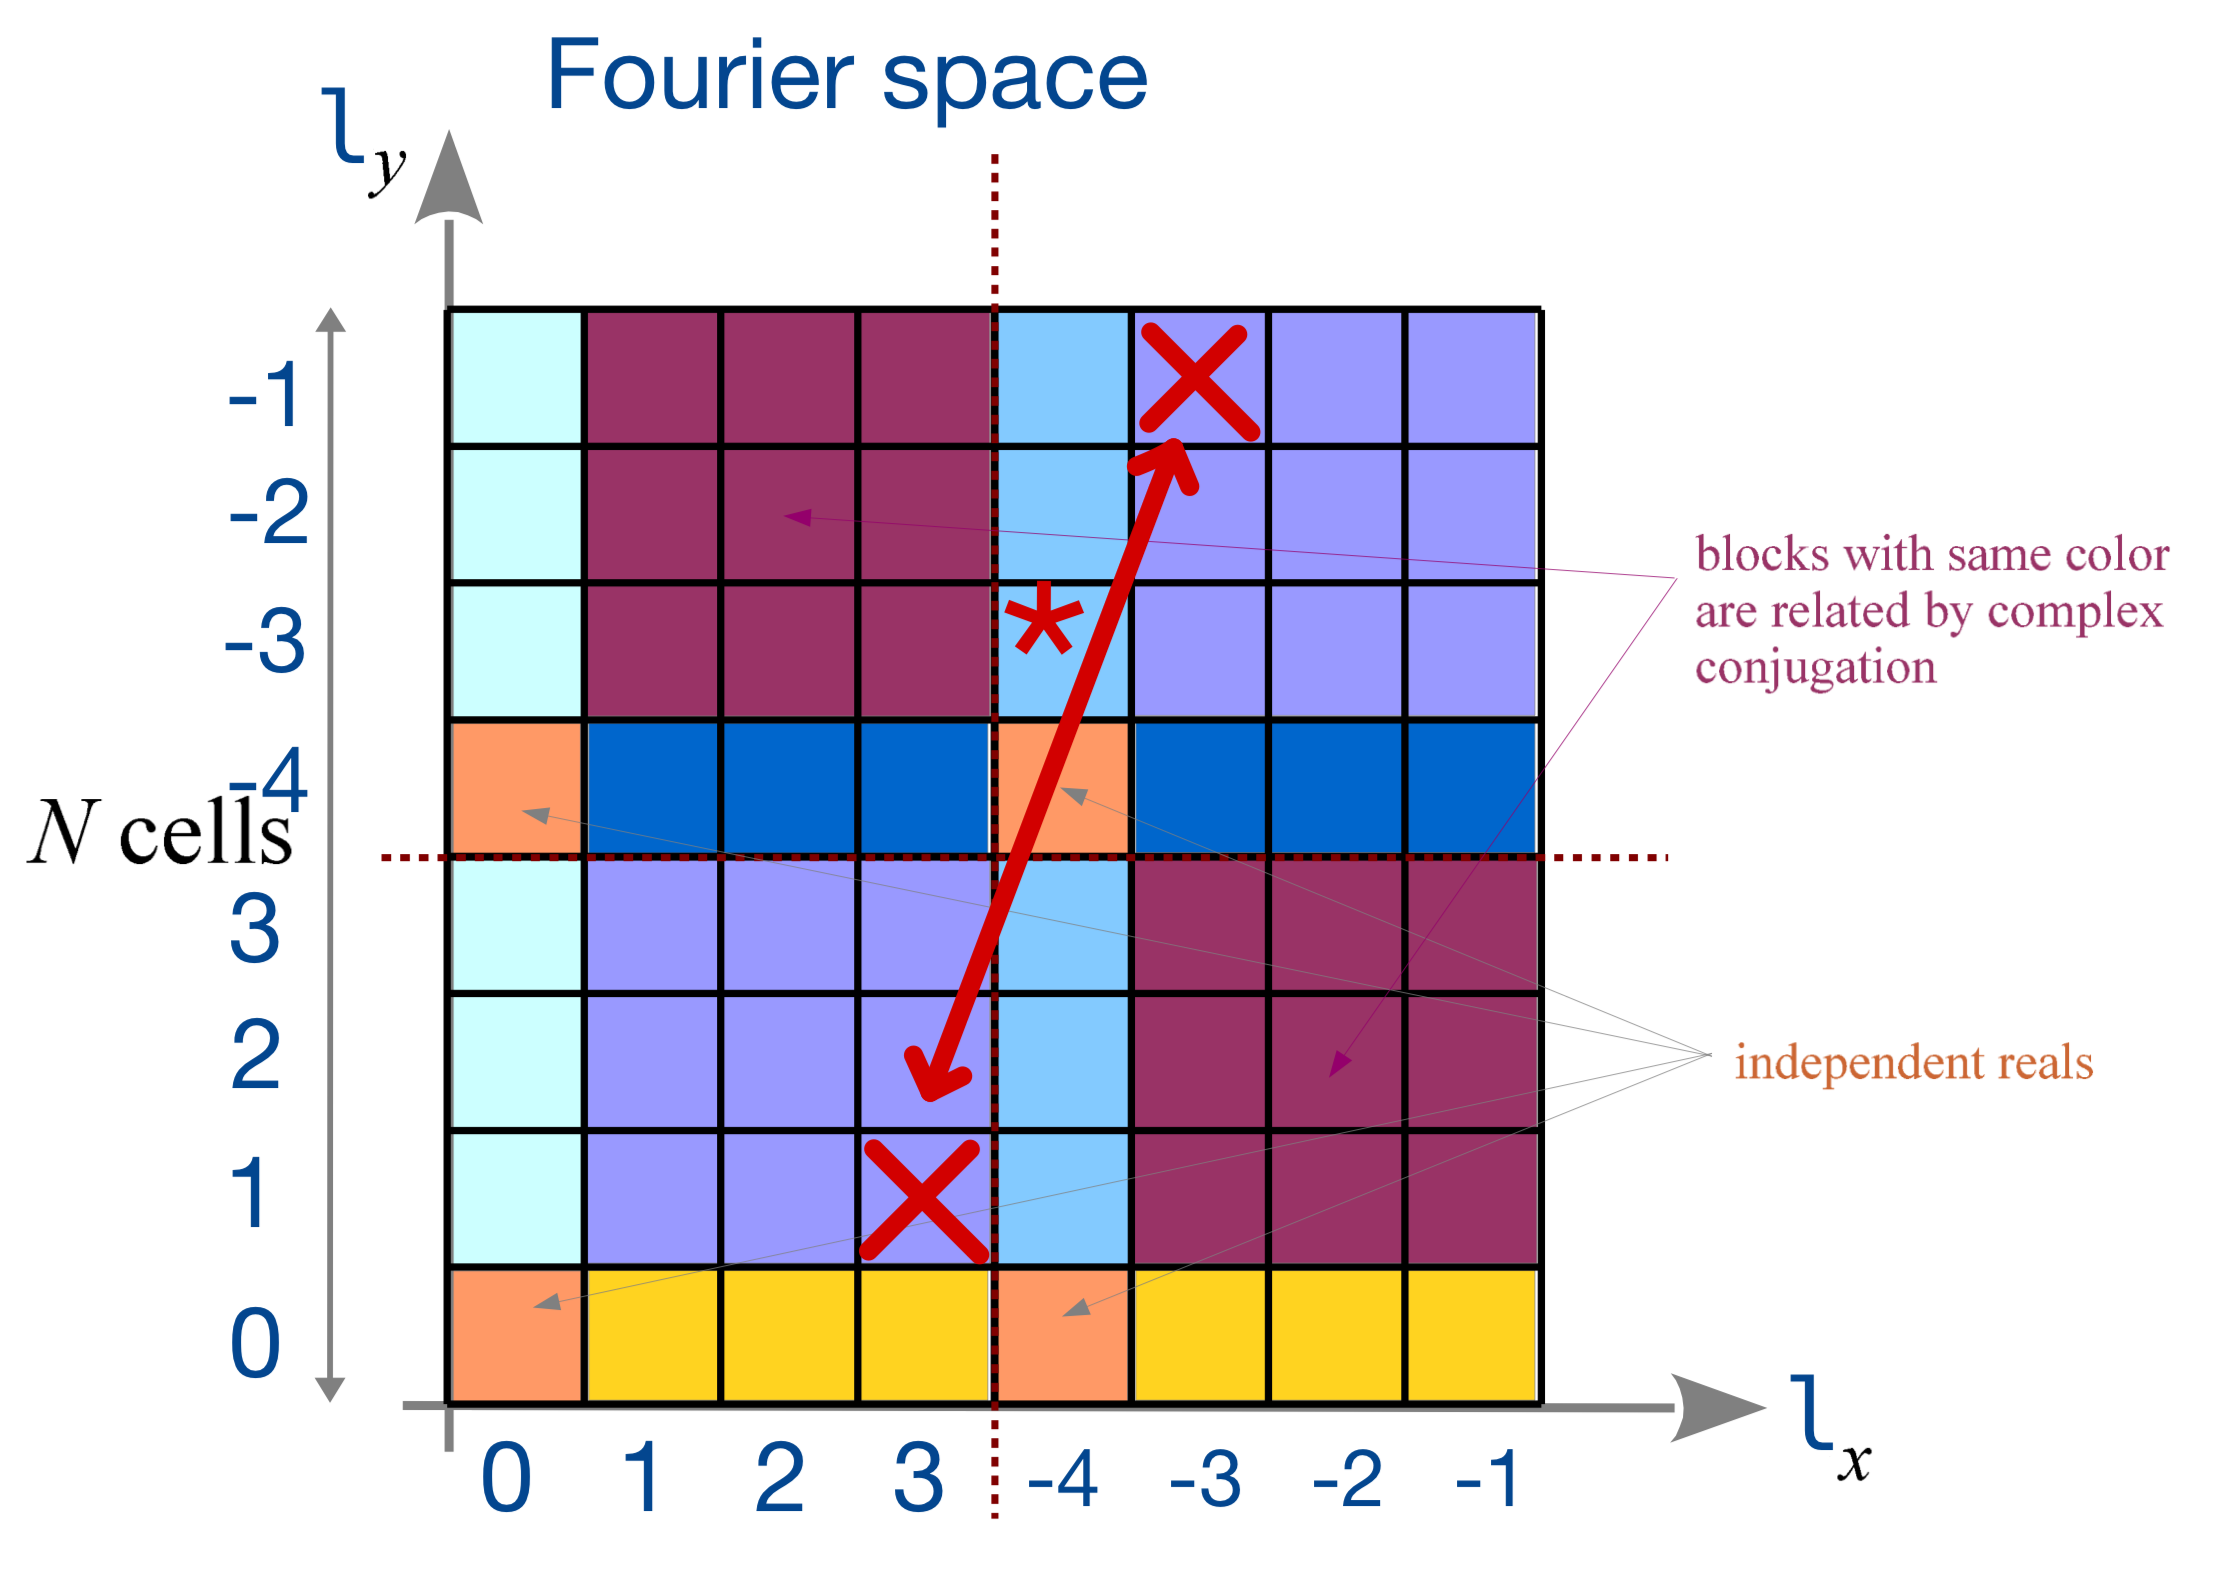
\includegraphics[width=0.9\textwidth]{figures/dftstorage2D.png}
    \caption{2D fourier space storage convention. Note that if the data in real space
    is real $\rho_{\vec{p}} \in \mathbb{R}$, then $\hat{\rho}_{\vec{l}} = \hat{\rho}_{-\vec{l}}^*$.
    Because of aliasing $\hat{\rho}_{-\frac{N}{2}} = \hat{\rho}_{\frac{N}{2}} = \hat{\rho}_{-\frac{N}{2}}^*$ so $\in \mathbb{R}$,
    marked in orange in the illustration. We have (a complex number consists of two independent real numbers) the same number of independent numbers as in real space.}
    \label{fig:dftstorage2D}
\end{figure}

\subsection{DFT and Linear and Cyclic Convolution}
Let us step back to the convolution of two functions - 
e.g. for solving the Poisson equation or for smoothing
an image. The convolution is defined as

\begin{equation}
    (f \star g)(t) = \int_{\mathbb{R}} f(\tau) g(t-\tau) d \tau
\end{equation}

so naturally for discrete $f,g$, we define

\begin{equation}
    (f * g)[n]=\sum_{m=-\infty}^{\infty} f[m] g[n-m]
\end{equation}

The basic intuition for convolutions is that one function is flipped and slides over the other
as a window, as illustrated in figure \ref{fig:convolution}.

\begin{figure}[ht]
    \centering
    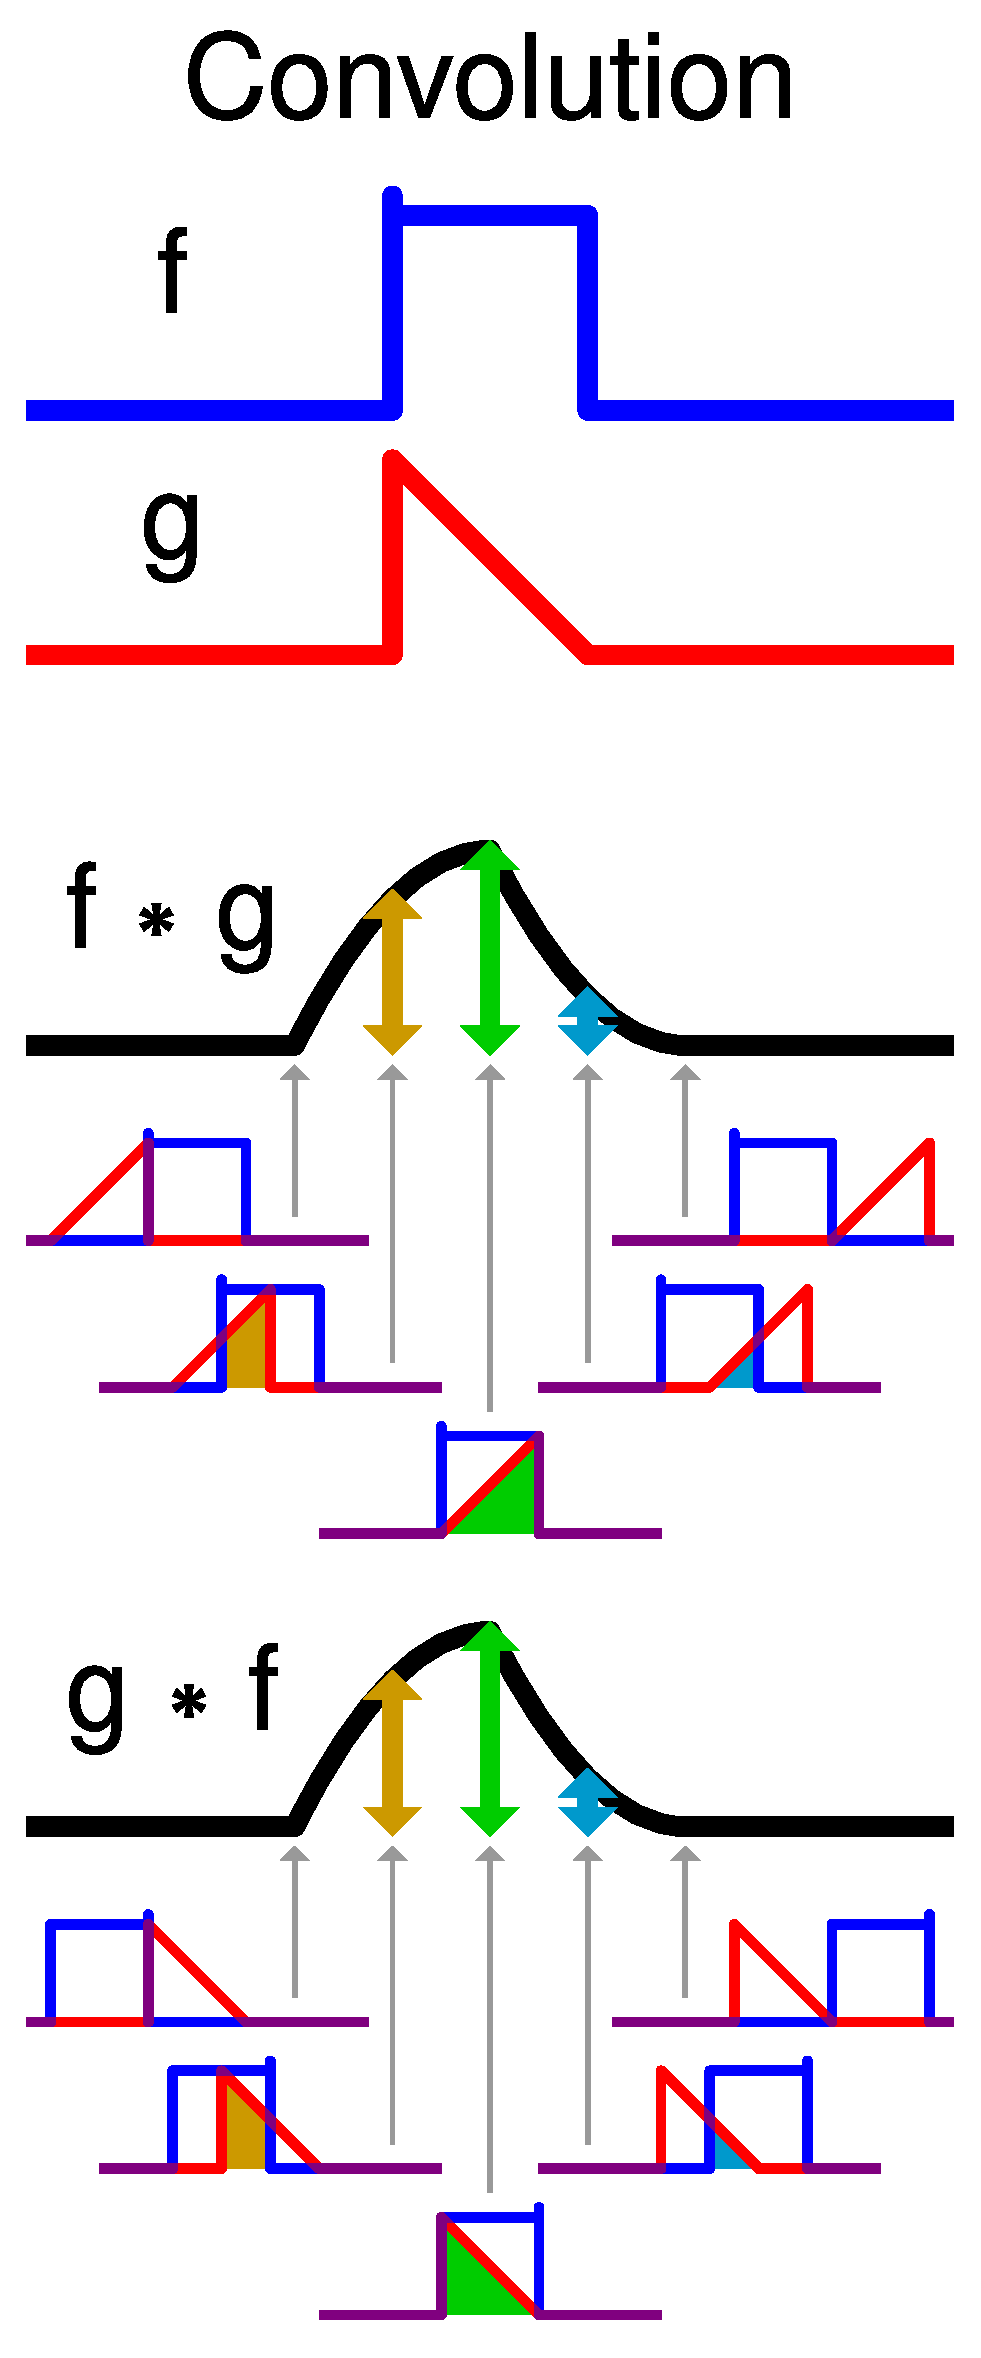
\includegraphics[width=0.5\textwidth]{figures/conv.pdf}
    \caption{Basic intuition for convoltions.}
    \label{fig:convolution}
\end{figure}

\note{When one convolves using $\text{ifft}(\text{fft}(f) \cdot \text{fft}(g))$ this is actually the
cyclic convolution
\begin{equation}
    \left(f * g_N\right)[n]=\sum_{m=0}^{N-1} f[m] g_N[n-m]
\end{equation}
assuming $f,g$ are periodic with period $N$. The wanted result from a linear convolution
is illustrated in figure \ref{fig:linear_convolution}, what we get from the cyclic convolution
is illustrated in figure \ref{fig:cyclic_convolution}. Code for the cyclic convolution
is given in code \ref{code:cyclic_convolution}.
}

\idea{If we zero-pad sufficiently, the cyclic convolution becomes a linear convolution. For two vectors
$\vec{f}$ of length $N$ and $\vec{g}$ of length $M$ we append zeros to both so they are 
both of length $N+M-1$ (the length of the linear convolution), see figure \ref{fig:cyclic_linear_convolution} and
code \ref{code:linear_convolution}.}

\begin{figure}
    \centering
    \includesvg[width=0.9\textwidth]{figures/linear_convolution.svg}
    \caption{Example of a linear convolution.}
    \label{fig:linear_convolution}
\end{figure}

\begin{figure}
    \centering
    \includesvg[width=0.9\textwidth]{figures/cyclic_convolution.svg}
    \caption{Example of a cyclic convolution.}
    \label{fig:cyclic_convolution}
\end{figure}

\begin{figure}
    \centering
    \includesvg[width=0.9\textwidth]{figures/cyclic_convolution_zero.svg}
    \caption{Illustration of the cyclic convolution becoming a linear convolution
    by zero-padding.}
    \label{fig:cyclic_linear_convolution}
\end{figure}


\begin{codebox}
    \begin{minted}{julia}
        # cyclic convolution in real space
        function DirectCyclicConv1D(f,g)
            N = length(f)
            Conv = zeros(N)  

            for n in 1:N, m in 1:N
                if n-m+1 > 0
                    Conv[n] = Conv[n] + f[m] * g[n-m+1]
                else
                    # make g periodic
                    Conv[n] = Conv[n] + f[m] * g[N+(n-m+1)]
                end
            end

            return Conv

        end

        # cyclic convolution in Fourier space
        FastCyclicConv1D(f,g) = ifft(fft(f).*fft(g))
    \end{minted}
    \caption{Cyclic convolution in Julia.}
    \label{code:cyclic_convolution}
\end{codebox}

\begin{codebox}
    \begin{minted}{julia}
        # simple linear convolution in real space
        function conv1d(f, g)
            n = length(f)
            m = length(g)
            y = zeros(n + m - 1)
            for i in 1:n
                for j in 1:m
                    y[i + j - 1] += f[i] * g[j]
                end
            end
            return y
        end

        # zero padded linear convolution in real space
        # note that this zero padded version is equivalent
        # to the cyclic convolution with zero padding
        function DirectLinearConvolution(f,g)
            N = length(f)
            M = length(g)

            g_pad = [ g; zeros(N-1) ]     # length N+M-1
            f_pad = [ f; zeros(M-1) ]     # length N+M-1

            Conv = zeros(N+M-1)
            for n=1:N+M-1
                for m=1:N+M-1
                    if n-m+1 > 0
                        Conv[n] = Conv[n] + f_pad[m] * g_pad[n-m+1]
                    end
                    # n+1 <= m
                end
            end
            return Conv
        end

        # fast linear convolution in Fourier space
        function FastLinearConvolution(f,g)
            N = length(f)
            M = length(g)
            f_pad = [ f; zeros(M-1) ]     
            g_pad = [ g; zeros(N-1) ]     
            return FastCyclicConv1D( f_pad, g_pad )
        end
    \end{minted}
    \caption{Linear convolution in Julia.}
    \label{code:linear_convolution}
\end{codebox}

\subsection{Non-periodic problems with \textit{zero-padding} in 2D}
\problem{DFT / FFT are defined for periodic problems, a convolution based on them is a cyclic convolution.}
\idea{As before we can zero-pad. \textcolor{red1}{The cost, however, rises ($\times 4$ in 2D).}}

For solving the Poisson equation for non-periodic density distributions, we
\begin{enumerate}
    \item set up the mesh so that the density distribution only lives in one quarter - rest zeroes (see figure \ref{fig:zero_padding_2D}).
    \item periodically extend the Green's function over the whole grid (so that the distance used is the one to the nearest periodic image)
    \begin{equation}
        g_{N-i,j} = g_{i,N-j} = g_{N-i,N-j} = g_{i,j}, \quad 0 \leq i,j \leq \frac{N}{2}
    \end{equation}
    which is symmetric around the origin (when replicating the mesh in all directions). \textcolor{red1}{Why does the Greens function have to be extended?}
    \item calculate $\phi = g \star \rho$, in real space this would be
    \begin{equation}
        \phi_\vec{p} = \sum_{\vec{n}} g_{\vec{p}-\vec{n}} \rho_\vec{n}, \quad \vec{g}, \vec{\rho} \text{ periodic in the index } N
    \end{equation}
    The zero padding is large enough so that if \textit{the Green's function slides over the density, there is no cross talk between periodic images of the density distribution}.
    We use the fast cyclic convolution in Fourier space.
\end{enumerate}

\begin{figure}[ht]
    \centering
    \includesvg[width=0.9\textwidth]{figures/zp3.svg}
    \caption{Illustration of the zero padding in 2D.}
    \label{fig:zero_padding_2D}
\end{figure}

\subsection{Power spectra and correlation functions}
Power spectra and correlation functions are deeply connected via the Fourier transform.
\textcolor{blue1}{Assume the field $\rho$ to be isotropic and homogeneous (mean or variance do not change under rotations and tranlations).}

\subsubsection{Definition of the power spectrum}
Consider the fourier transform (decomposing the scaler field $\rho$ into plane waves)
\begin{equation}
    \rho(\vec{x})=\frac{1}{(2 \pi)^3} \int \hat{\rho}(\vec{k}) e^{-i \vec{k} \cdot \vec{x}} d^3 \vec{k}, \quad \hat{\rho}(\vec{k})=\int \rho(\vec{x}) e^{i \vec{k} \cdot \vec{x}} d^3 \vec{x}
\end{equation}
the variance in Fourier space defines the power spectrum $P(k)$
\begin{equation}
    \label{eq:powerspectrum}
    \left\langle\hat{\rho}(\vec{k}) \hat{\rho}^*\left(\vec{k}^{\prime}\right)\right\rangle \equiv(2 \pi)^3 P(k) \delta\left(\vec{k}-\vec{k}^{\prime}\right), \quad k=|\vec{k}|, \quad \text { (isotropic) power spectrum } P
\end{equation}
- modes with different wave vector are uncorrelated (ensured by Delta distribution) to ensure homogeneity. To ensure
isotropy, the power spectrum $P$ cannot depend on the direction of $\vec{k}$.

\yellowbox{Usually the energy spectral density for a measurement $x(t)$ over time is just $\bar{S}_{x x}(f) \triangleq|\hat{x}(f)|^2$ where $f$ is a frequency (Fourier transform in time) and
the general signal processing understanding of energy as $E \triangleq \int_{-\infty}^{\infty}|x(t)|^2 d t$ is used (which based on Plancherel's theorem $\int_{-\infty}^{\infty}|x(t)|^2 d t=\int_{-\infty}^{\infty}|\hat{x}(f)|^2 d f$ makes the formula for the \textit{spectral} energy density (in a small frequency interval) plausible).}

\subsubsection{Definition of the correlation function}
The auto-correlation function
\begin{equation}
    \begin{gathered}
        \xi(y)=\langle\rho(\vec{x}) \rho(\vec{x}+\vec{y})\rangle \\
        \text{average over all positions } \vec{x} and \text{\textbf{orientations} of } \vec{y}
    \end{gathered}
\end{equation}
measures the coherence of the fluctuating field $\rho$ at all
points seperated by $\vec{y}$ (can also not depend on the
direction of $\vec{y}$ as of isotropy). For $\vec{y} = 0$ we have the variance.

\subsubsection{Connection by Fourier Transform}
Correlation function and power spectrum are Fourier transforms of each
other (can be seen by inserting the Fourier tranforms into the
correlation function), hence carry an equivalent amount of information.

From this we can find the variance of $\rho$ in real space (at $y = 0$) to be

\begin{equation}
    \label{eq:variance_kspace}
    \sigma^2 = \frac{4\pi}{(2 \pi)^3} \int P(k) k^2 \, dk
\end{equation}

\subsubsection{Power function and variance of a smoothed field}
Consider the smoothed field
\begin{equation}
    \bar{\rho}(\vec{x}) = \int \rho(\vec{y}) W_R(||\vec{x}-\vec{y}||) \, d^3 \vec{y}, \quad \text{window with compact support } R
\end{equation}
which is a convolution. As of the convolution theorem $\widehat{f \star g} = \hat{f} \hat{g}$, we have
\begin{equation}
    \hat{\bar{\rho}}(\vec{k}) = \hat{\rho}(\vec{k}) \hat{W}_R(\vec{k})
\end{equation}
so the power spectrum (as of eq. \ref{eq:powerspectrum}) of the smoothed field is
\begin{equation}
    \bar{P}(k) = P(k) \hat{W}_R^2(k)
\end{equation}
which can be used to calculate a variance of the smoothed field using eq. \ref{eq:variance_kspace}.

\subsection{Projections in Fourier space}
\greenbox{Splitting a vector field into a source-free rotational and a curl-free part can be useful (e.g. for cleaning divergence from a
numerically obtained magnetic field) - this can be done and proven in Fourier space.}
One can proof the Helmholtz decomposition (fundamental theorem of vector analysis) using Fourier transform.

\subsubsection{Fundamental theorem of vector analysis | Helmholtz decomposition}
Let $\vec{F}(\vec{x})$ be a vector field with compact support and derivatives that vanish at infinity.

Then $\vec{F}$ can be uniquely decomposed into a curl-free (longitudinal, purely radial in Fourier space) and a divergence-free part

\begin{equation}
    \begin{gathered}
        \vec{F}(\vec{x}) = \vec{F}_\perp(\vec{x}) + \vec{F}_\parallel(\vec{x}) \\
        \vec{\nabla} \cdot \vec{F}_\perp = 0, \quad \vec{\nabla} \times \vec{F}_\parallel = 0
    \end{gathered}
\end{equation}

\subsubsection{Proof in Fourier space}
Consider a decomposition of the Fourier transform $\hat{\vec{F}}(\vec{k})$ of $\vec{F}(\vec{x})$ into a part parallel
and perpendicular to $\vec{k}$ (the wave vector)

\begin{equation}
    \begin{gathered}
        \hat{\vec{F}}(\vec{k}) = \hat{\vec{F}}_\perp(\vec{k}) + \hat{\vec{F}}_\parallel(\vec{k}) \\
        \hat{\vec{F}}_\parallel(\vec{k}) = \vec{\hat{e}}_k \left( \vec{\hat{e}}_k \cdot \hat{\vec{F}}(\vec{k}) \right), \quad \vec{\hat{e}}_k = \frac{\vec{k}}{||\vec{k}||}  \\
        \hat{\vec{F}}_\perp(\vec{k}) = \hat{\vec{F}}(\vec{k}) - \hat{\vec{F}}_\parallel(\vec{k})
    \end{gathered}
\end{equation}

In Fourier space divergence and curl are simple to calculate (they become scalar products and cross products with $\vec{k}$ respectively).

\begin{equation}
    \vec{k} \cdot \hat{\vec{F}}_\perp(\vec{k}) = 0, \quad \vec{k} \times \hat{\vec{F}}_\parallel(\vec{k}) = 0
\end{equation}

from which by inverse Fourier transform the Helmholtz decomposition follows.

\subsubsection{Applications of the Helmholtz decomposition}
\begin{itemize}
    \item Retain $\vec{\nabla} \cdot \vec{B} = 0$ in simulations by projecting out the radial component (the one with divergence in real space) in Fourier space ($\vec{\hat{B}}(\vec{k}) \rightarrow \vec{\hat{B}}(\vec{k}) - \vec{\hat{e}}_k \vec{\hat{e}}_k  \cdot \vec{\hat{B}}(\vec{k})$, then apply inverser Fourier transform to get the source-clensed field).
    \item Analyze turbulent flow for shocks
    \item Stability analysis in astrophysics: Based on determining how much compressive motion and how much solenoidal motion is present, stability can be analyzed. Solenoidal motion stabilizes, compressive motion increases density so astrophysically the cooling rate of the system ($\propto \rho^2$) and finally leads to collapse.
    This can be studied by Fourier transform (problem: spatial information is non-local in Fourier space), and also based on
    \begin{equation}
        \partial_t \rho = - \rho \vec{\nabla} \cdot \vec{v}, \quad \text{solenoidal } \vec{\nabla} \cdot \vec{v} = 0 \rightarrow \partial_t \rho = 0
    \end{equation}
    which can be seen as a peak in the probability distribution of the density which is broader for compressive motion.
\end{itemize}

\subsubsection{Sidenote: Importance of dimensionality}
Depending on the dimensionality, we have
\begin{itemize}
    \item 1D: one compressible mode
    \item 2D: one compressible, one source-free (solenoidal, non-compressive) mode
    \item 3D: one compressible, two source-free modes
\end{itemize}

In a tube with small width we mostly have compressible modes, in shallow water we can have vortices with spin perpendicular to the surface.

\pagebreak